\documentclass[12pt,letterpaper]{article}
\usepackage[utf8]{inputenc}
\usepackage[spanish]{babel}
\usepackage{graphicx}
\usepackage[left=2cm,right=2cm,top=2cm,bottom=2cm]{geometry}
\usepackage{graphicx} % figuras
% \usepackage{subfigure} % subfiguras
\usepackage{float} % para usar [H]
\usepackage{amsmath}
%\usepackage{txfonts}
\usepackage{stackrel} 
\usepackage{multirow}
\usepackage{enumerate} % enumerados
\renewcommand{\labelitemi}{$-$}
\renewcommand{\labelitemii}{$\cdot$}
% \author{}
% \title{Caratula}
\begin{document}

% Fancy Header and Footer
% \usepackage{fancyhdr}
% \pagestyle{fancy}
% \cfoot{}
% \rfoot{\thepage}
%

% \usepackage[hidelinks]{hyperref} % CREA HYPERVINCULOS EN INDICE

% \author{}
\title{Caratula}

\begin{titlepage}
\begin{center}
\large{UNIVERSIDAD PRIVADA DE TACNA}\\
\vspace*{-0.025in}
\begin{figure}[htb]
\begin{center}

\includegraphics[width=4cm]{./Imagenes/logo}
\end{center}
\end{figure}
\vspace*{0.15in}
INGENIERIA DE SISTEMAS  \\

\vspace*{0.5in}
\begin{large}
TEMA:\\
\end{large}

\vspace*{0.1in}
\begin{Large}
\textbf{Test-Driven Development} \\
\end{Large}

\vspace*{0.3in}
\begin{Large}
\textbf{CURSO:} \\
\end{Large}

\vspace*{0.1in}
\begin{large}
BASE DE DATOS II\\
\end{large}

\vspace*{0.3in}
\begin{Large}
\textbf{DOCENTE(ING):} \\
\end{Large}

\vspace*{0.1in}
\begin{large}
 Patrick Jose Cuadros Quiroga\\
\end{large}

\vspace*{0.2in}
\vspace*{0.1in}
\begin{large}
Integrantes: \\
\begin{flushleft}

Wilfredo Vilca Chambilla          	\hfill	(2006028540) \\

\end{flushleft}
\end{large}
\end{center}

\end{titlepage}


\tableofcontents % INDICE
\thispagestyle{empty} % INDICE SIN NUMERO
\newpage
\setcounter{page}{1} % REINICIAR CONTADOR DE PAGINAS DESPUES DEL INDICE

\section{Ejercicio 1: Escribiendo consultas con el operador PIVOT} 
\textbf{}\\
\textbf{Tarea 1: Escriba una declaración SELECT para recuperar el número de clientes para un específico grupo de clientes}
\textbf{}\\
\textbf{}\\
Paso 1. Inicie SQL Server Management Studio y conéctese al motor de base de datos (local) usando Windows autenticación.

\begin{flushleft}

\begin{center}
	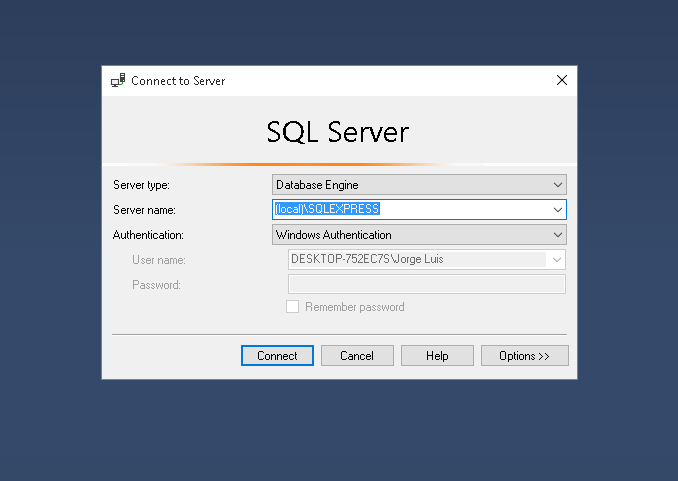
\includegraphics[width=10cm]{./Imagenes/img1} 
	\end{center}


Paso 2. En el menú Archivo, haga clic en Abrir y haga clic en Proyecto / Solución.

\begin{center}
	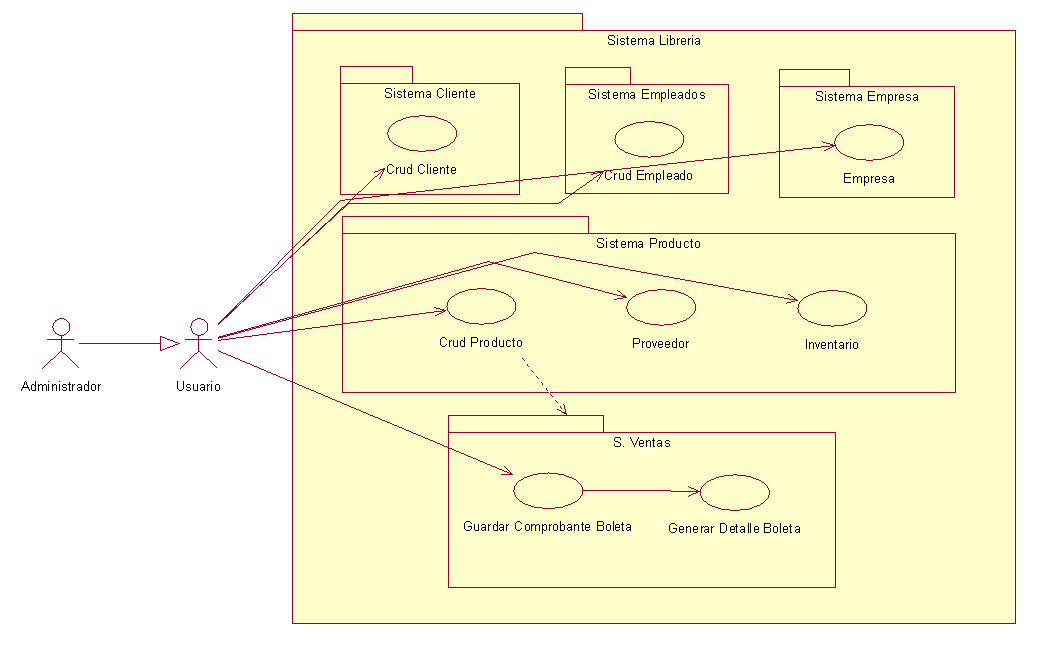
\includegraphics[width=10cm]{./Imagenes/img2} 
	\end{center}

\textbf{}\\
\textbf{}\\
\textbf{}\\
\textbf{}\\
\textbf{}\\
\textbf{}\\
\textbf{}\\
\textbf{}\\
\textbf{}\\
Paso 3. En la ventana Abrir proyecto, abra el proyecto Proyecto.ssmssln.
\begin{center}
	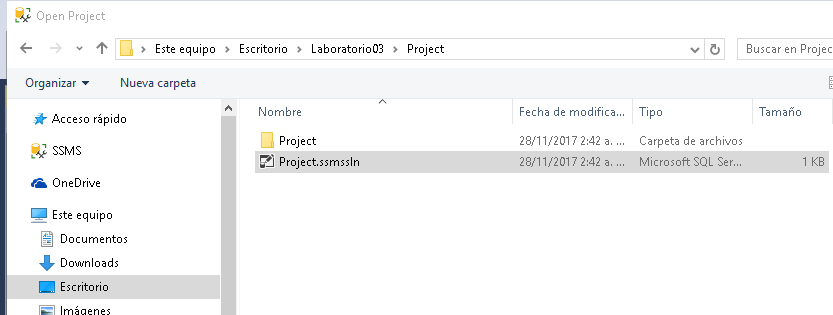
\includegraphics[width=10cm]{./Imagenes/img3} 
	\end{center}

Paso 4. En el Explorador de soluciones, haga doble clic en la consulta 51 - Ejercicio de laboratorio 1.sql.
\begin{center}
	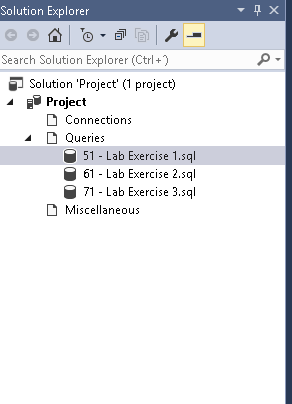
\includegraphics[width=10cm]{./Imagenes/img4} 
	\end{center}
\textbf{}\\
\textbf{}\\
\textbf{}\\

\textbf{}\\
\textbf{}\\
Paso 5. En la ventana de consulta, resalte la instrucción USE TSQL; y haga clic en Ejecutar.
\begin{center}
	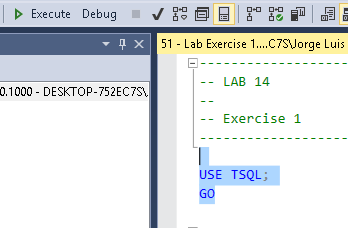
\includegraphics[width=10cm]{./Imagenes/img5} 
	\end{center}

Paso 6. Resalte el siguiente código T-SQL proporcionado:

\begin{center}
	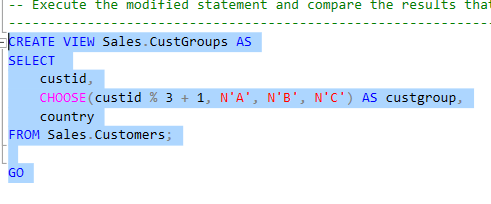
\includegraphics[width=10cm]{./Imagenes/img6} 
	\end{center}

Paso 7. Haga clic en Ejecutar. Este código crea una vista llamada Sales.CustGroups
\begin{center}
	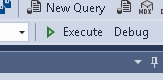
\includegraphics[width=10cm]{./Imagenes/img7} 
	\end{center}
\begin{center}
	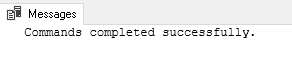
\includegraphics[width=10cm]{./Imagenes/img71} 
	\end{center}

Paso 8. En el panel de consulta, escriba la siguiente consulta después del código T-SQL proporcionado:
\textbf{}\\
\textbf{}\\
SELECT\\
custid,\\
custgroup,\\
country\\
FROM Sales.CustGroups;\\

\textbf{}\\
Paso 9. Resalte la consulta escrita y haga clic en Ejecutar.
\begin{center}
	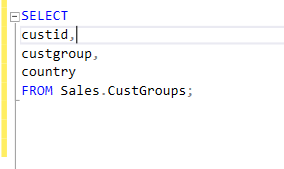
\includegraphics[width=5cm]{./Imagenes/img9} 
	\end{center}
\begin{center}
	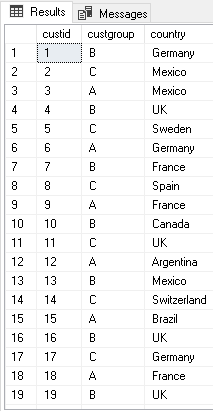
\includegraphics[width=5cm]{./Imagenes/img91} 
	\end{center}


Paso 10. Modifique el código T-SQL escrito aplicando el operador PIVOT. La consulta debería verse así:
\textbf{}\\
\textbf{}\\
SELECT\\
country,\\
p.A,\\
p.B,\\
p.C\\
FROM Sales.CustGroups\\
PIVOT (COUNT(custid) FOR custgroup IN (A, B, C)) AS p;\\

Paso 11. Resalte la consulta escrita y haga clic en Ejecutar.
\textbf{}\\
\begin{center}
	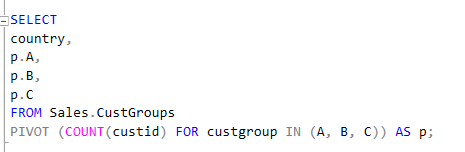
\includegraphics[width=8cm]{./Imagenes/img11} 
	\end{center}
\begin{center}
	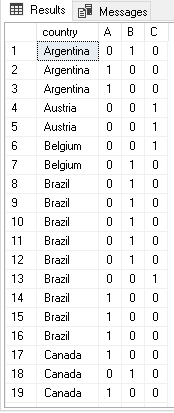
\includegraphics[width=5cm]{./Imagenes/img111} 
	\end{center}

\textbf{Tarea 2: Especifique el elemento de agrupación para el operador PIVOT}
\textbf{}\\
\textbf{}\\
Paso 1. Resalte el siguiente código T-SQL proporcionado después de la descripción de la Tarea 2:
\begin{center}
	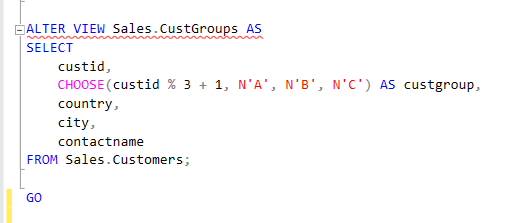
\includegraphics[width=10cm]{./Imagenes/2img1} 
	\end{center}
\textbf{}\\
\textbf{}\\
\textbf{}\\
\textbf{}\\
Paso 2. Haga clic en Ejecutar. Este código modifica la vista agregando dos columnas adicionales.
\begin{center}
	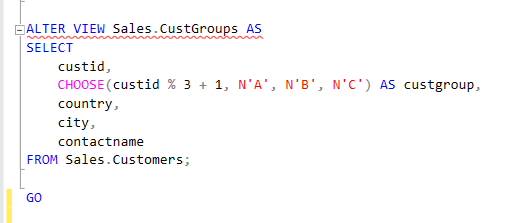
\includegraphics[width=10cm]{./Imagenes/2img1} 
	\end{center}


Paso 3. Resalte la última consulta en la tarea 1. En la barra de herramientas, haga clic en Editar y luego en Copiar
\textbf{}\\
\textbf{}\\
SELECT\\
country,\\
p.A,\\
p.B,\\
p.C\\
FROM Sales.CustGroups\\
PIVOT (COUNT(custid) FOR custgroup IN (A, B, C)) AS p;\\

\textbf{}\\
\textbf{}\\


Paso 4. En la ventana de consulta, haga clic en la línea después del código T-SQL proporcionado. En la barra de herramientas, haga clic en Editar y luego en Pegar.
\begin{center}
	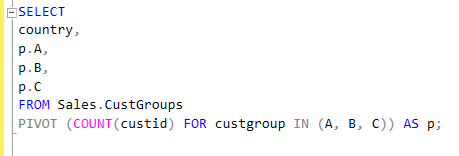
\includegraphics[width=10cm]{./Imagenes/2img4} 
	\end{center}

Paso 5. Resalte la consulta copiada y haga clic en Ejecutar.
\begin{center}
	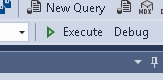
\includegraphics[width=10cm]{./Imagenes/2img5} 
	\end{center}
\textbf{}\\
\textbf{}\\

Paso 6. Observa el resultado. ¿Es este resultado el mismo que el de la consulta en la tarea 1?\\
\textbf{}\\
- El resultado no es el mismo. Más filas fueron devueltas después de que modificó la vista.
\textbf{}\\
\textbf{}\\

Paso 7. Modifique la sentencia T-SQL copiada para incluir columnas adicionales de la vista. La consulta debe se parece a esto:\\
\textbf{}\\
SELECT\\
country,\\
city,\\
contactname,\\
p.A,\\
p.B,\\
p.C\\
FROM Sales.CustGroups\\
PIVOT (COUNT(custid) FOR custgroup IN (A, B, C)) AS p; \\
\textbf{}\\
\textbf{}\\
Paso 8. Resalte la consulta escrita y haga clic en Ejecutar.
\begin{center}
	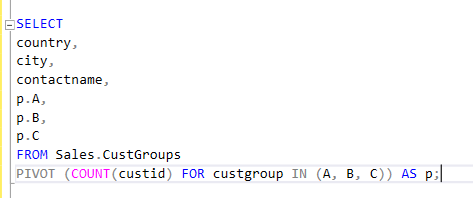
\includegraphics[width=10cm]{./Imagenes/2img8} 
	\end{center}

\begin{center}
	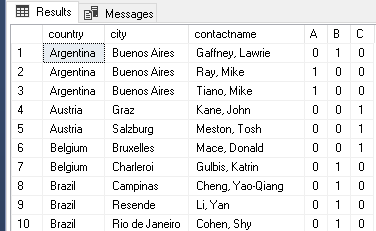
\includegraphics[width=10cm]{./Imagenes/2img81} 
	\end{center}
\textbf{}\\
\textbf{}\\
Paso 9. Observe que recibió el mismo resultado que la consulta anterior. ¿Por qué obtuviste el mismo número de filas?\\
- El operador PIVOT asume que todas las columnas, excepto la agregación y la propagación
Los elementos forman parte de las columnas de agrupación.


\textbf{Tarea 3: usar una expresión de tabla común (CTE) para especificar el elemento de agrupación para el operador PIVOT}
\textbf{}\\
\textbf{}\\

Paso 1. En el panel de consulta, escriba la siguiente consulta después de la descripción de la Tarea 3:
\textbf{}\\
\textbf{}\\
WITH PivotCustGroups AS\\
(\\
SELECT\\
custid,\\
country,\\
custgroup\\
FROM Sales.CustGroups\\
)\\
SELECT\\
country,\\
p.A,\\
p.B,\\
p.C\\
FROM PivotCustGroups\\
PIVOT (COUNT(custid) FOR custgroup IN (A, B, C)) AS p;\\
\textbf{}\\
\textbf{}\\
Paso 2. Resalte la consulta escrita y haga clic en Ejecutar
\begin{center}
	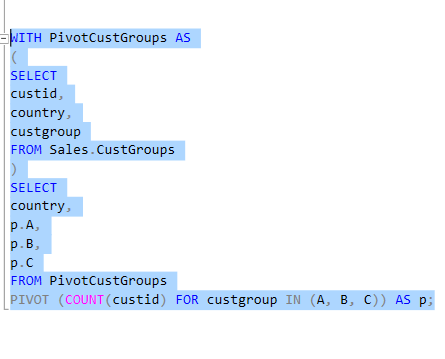
\includegraphics[width=10cm]{./Imagenes/3img1} 
	\end{center}

\textbf{}\\
\textbf{}\\
\textbf{}\\
\textbf{}\\
\textbf{}\\
\textbf{}\\
Paso 3. Observa el resultado. ¿Es el mismo que el resultado de la última consulta en la tarea 1? ¿Puedes explicar por qué? \\
\textbf{}\\
- El resultado es el mismo. En esta tarea, el CTE ha proporcionado tres columnas posibles al operador PIVOT. En tarea 1, la vista también proporcionó tres columnas al operador PIVOT.
\textbf{}\\
\begin{center}
	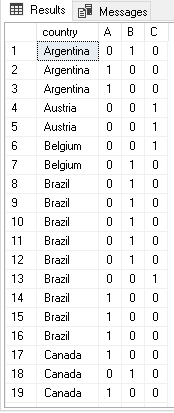
\includegraphics[width=4cm]{./Imagenes/3img3} 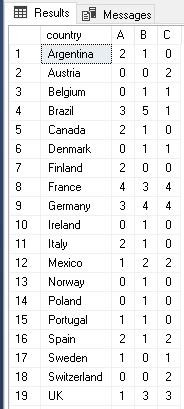
\includegraphics[width=4cm]{./Imagenes/3img31} 
	\end{center}

Paso 4. ¿Por qué cree que es beneficioso utilizar un CTE cuando se usa el operador PIVOT? \\
\textbf{}\\
Al usar el operador PIVOT, usted no puede especificar directamente el elemento de agrupación porque SQL Server automáticamente asume que todas las columnas deben usarse como elementos de agrupación, con la excepción de la propagación y elementos de agregación. Con un CTE, puede especificar las columnas exactas y, por lo tanto, controlar que Columnas utilizadas para la agrupación.
\textbf{}\\
\textbf{}\\
\textbf{}\\
\textbf{}\\
\textbf{}\\
\textbf{}\\

\textbf{}\\
\textbf{}\\
\textbf{}\\
\textbf{}\\
\textbf{}\\
\textbf{Tarea 4: Escriba una instrucción SELECT para recuperar el monto total de ventas para cada uno de Categoría de cliente y producto}
\textbf{}\\
\textbf{}\\

Paso 1. En el panel de consulta, escriba la siguiente consulta después de la descripción de la Tarea 4.
\textbf{}\\
\textbf{}\\
\begin{center}
	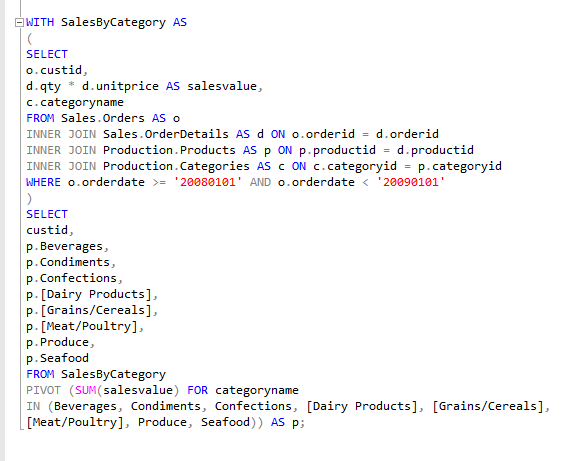
\includegraphics[width=10cm]{./Imagenes/4img1}
	\end{center}
\textbf{}\\
\textbf{}\\
Paso 2. Resalte la consulta escrita y haga clic en Ejecutar.
\textbf{}\\
\textbf{}\\
\begin{center}
	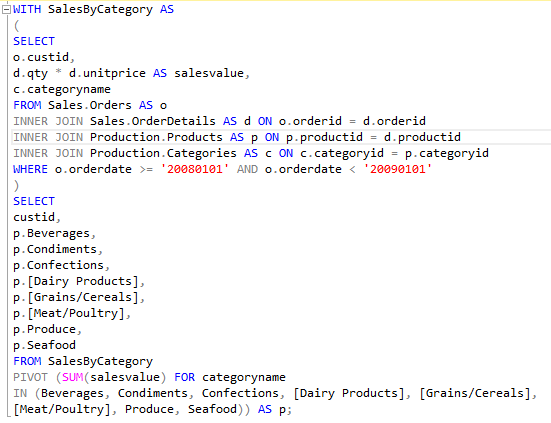
\includegraphics[width=10cm]{./Imagenes/4img2}
	\end{center}
\textbf{}\\
\textbf{}\\
\begin{center}
	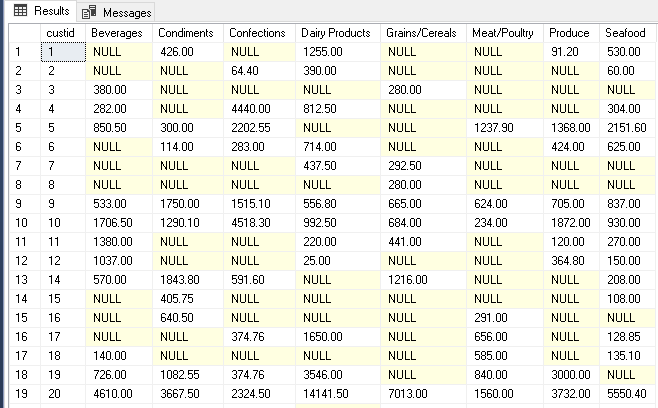
\includegraphics[width=10cm]{./Imagenes/4img3}
	\end{center}








\end{flushleft}
\section{¿Qué es Desarrollo Orientado A Pruebas (TDD)?} 
\textbf{}\\
Esta técnica llamada TDD (Test Driven Development), se puede definir como un proceso de desarrollo de software que se basa en la idea de desarrollar unas pequeñas pruebas, codificarlas y luego refactorizar el código que hemos implementado anteriormente.
Podemos decir que esta técnica e implementación de software está dentro de la metodología XP donde deberíamos de echarle un ojo a todas sus técnicas, tras leer varios artículos en un coincido con Peter Provost con un diseño dirigido o implementado a base de ejemplos hubiese sido mejor pero TDD se centra en 3 objetivos claros:

\begin{flushleft}

\begin{itemize}

	\item Una implementación de las funciones justas que el cliente necesita y no más, solamente las funciones que necesitamos, estoy cansado de duplicar dichas funciones para que hagan lo mismo

	 Mínimos defectos en fase de producción

	\item Producción de software modular y sobre todo reutilizable y preparado para el cambio


\textbf{}\\
Esta técnica se basa en la idea de realizar unas pruebas unitarias para un código que nosotros debemos construir, Nuestro TDD lo que nos dice es que primero los programadores debemos realizar una prueba y a continuación empezar a desarrollar el código que la resuelve.
El método que debemos seguir a para empezar a utilizar TDD es sencillo, Nos sirve para elegir uno de los requisitos a implementar, buscar un primer ejemplo sencillo, crear una prueba, ejecutarla e implementar el código mínimo para superar dicha prueba.
Obviamente la gracia de ejecutar la prueba después de crearla es ver que esta falla y que será necesario hacer algo en el código para que esta pase.
El ciclo de desarrollo de TDD es empezar la prueba, en test realizar un test, revisar el código y pasar el refactor.

\textbf {Crear la prueba o test}
\item Ejecutar los tests: falla (ROJO)
\item Crear código específico para resolver el test
\item Ejecutar de nuevo los tests: pasa (VERDE)
\item Refactorizar el código
\item Ejecutar los tests: pasa (VERDE)

\textbf {Personalmente, añadiría lo siguiente:}
\item Incrementa la productividad.
\item Nos hace descubrir y afrontar más casos de uso en tiempo de diseño.
\item La jornada se hace mucho más amena.
\item Uno se marcha a casa con la reconfortante sensación de que el trabajo está bien hecho.


Ahora bien, como cualquier técnica, no es una varita mágica y no dará el mismo resultado a un experto arquitecto de software que a un programador junior que está empezando. Sin embargo, es útil para ambos y para todo el rango de integrantes del equipo que hay entre uno y otro.
Es una técnica a tener en cuenta en el desarrollo web y sobre todo en el desarrollo de ingeniería software donde debemos tener en cuenta muchos fallos antes de pasar a producción.



\end{itemize} 


\end{flushleft}
\section{Patrones de Diseño Decorator} 

\textbf{}\\
“Añadir responsabilidades a un objeto de forma dinámica. Los decoradores proporcionan una alternativa flexible a la herencia para extender funcionalidad.”

\begin{center}
	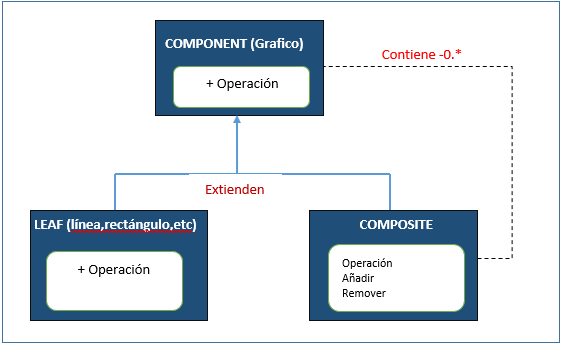
\includegraphics[width=10cm]{./Imagenes/composite1} 
	\end{center}


\begin{flushleft}

El siguiente de los patrones estructurales que veremos sera el patrón Decorator o decorador. Su filosofía consiste en añadir responsabilidades de forma dinámica con el principal objetivo de evitar la conocida como “explosión de clases”, es decir, la generación de un número elevado de subclases a partir de una superclase común.
Como podemos observar en el gráfico superior, la clase Decorator hereda de la misma clase que el componente que se quiere decorar. Así, cada decorador es capaz de encapsular una instancia de cualquier otro objeto que herede del componente común, bien un componente concreto u otro decorador. Este comportamiento recuerda al que vimos previamente en el patrón Adapter, con la diferencia de que la clase Decorator, a diferencia de la clase Adapter, no transforma una interfaz, sino que añade cierta funcionalidad.
La encapsulación puede ser iterativa, de modo que un componente concreto puede ser encapsulado por un decorador, que a su vez puede ser encapsulado por otro decorador… y así sucesivamente, añadiendo nueva funcionalidad en cada uno de los pasos. Resumiendo: el patrón Decoratorsustituye la herencia por un proceso iterativo de composición.


\begin{center}
	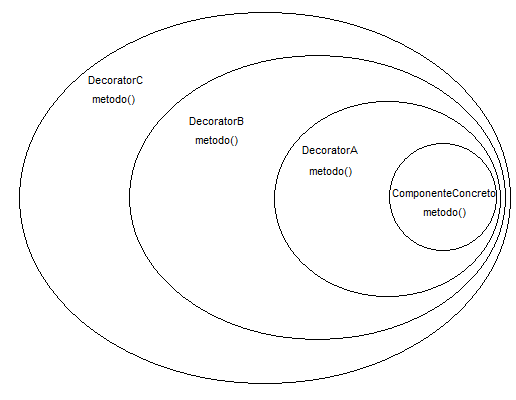
\includegraphics[width=10cm]{./Imagenes/decorator2} 
	\end{center}

El objeto con el que el objeto cliente interactuará será aquel que se encuentre en la capa más externa (en este caso, DecoratorC), que se encargará de acceder a los objetos contenidos e invocar su funcionalidad, que será devuelta a las capas exteriores.
Para comenzar, por tanto, debemos tener claros los siguientes conceptos sobre este patrón:

\begin{itemize}



  \item Un decorador hereda de la misma clase que los objetos que tendrá que decorar.
  \item Es posible utilizar más de un decorador para encapsular un mismo objeto.
\item El objeto decorador añade su propia funcionalidad, bien antes, bien después, de delegar el resto del trabajo en el objeto que está decorando.
\item Los objetos pueden decorarse en cualquier momento, por lo que es posible decorar objetos de forma dinámica en tiempo de ejecución.

\end{itemize} 

\textbf{}\\
La razón por la que la clase Decorator hereda de la misma clase que el objeto que tendrá que decorar no es la de añadir funcionalidad, sino la de asegurarse de que ambos comparten el mismo tipo y puedan intercambiarse: un decorador podrá sustituir a un objeto decorado, basándonos en el principio SOLID del Principio de sustitución de Liskov.


\textbf{Declarando las clases funcionales}

Como viene siendo habitual, ilustraremos nuestro patrón haciendo uso de vehículos. En este caso, utilizaremos una case abstracta, llamada Vehiculo, del que heredarán las clases funcionales a las que llamaremos “Berlina” y “Monovolumen”, y los decoradores, que se limitarán a añadir funcionalidad a estas clases funcionales. Los decoradores que diseñaremos serán “Diesel”, “Gasolina”, “Inyeccion”, “CommonRail” y “Turbo”.

Estos decoradores se caracterizarán por:

\begin{itemize}



  \item Disponer de una referencia a un vehículo que será inyectada en el constructor.
  \item Modificar el funcionamiento original de la clase que decoran, sobrecargando los métodos y llamando a los métodos de las clases encapsuladas para modificar su información o funcionamiento.


\end{itemize} 

\textbf{}\\ 
Comencemos codificando nuestra clase abstracta Vehiculo de la cual heredarán el resto de clases.

\begin{center}
	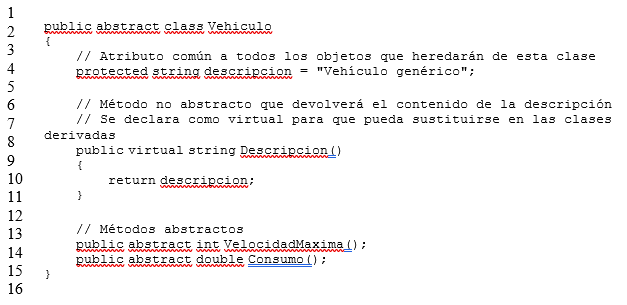
\includegraphics[width=10cm]{./Imagenes/decorator3} 
	\end{center}

Hecho esto, añadiremos nuestras clases funcionales: Monovolumen y Berlina.

\textbf{Monovolumen}
\begin{center}
	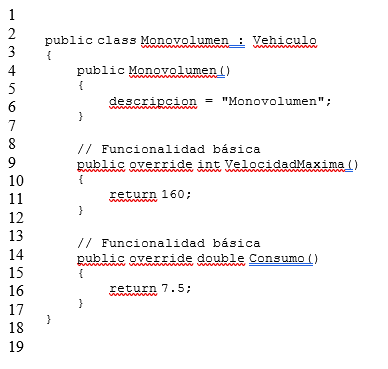
\includegraphics[width=10cm]{./Imagenes/decorator4} 
	\end{center}


\textbf{Berlina}
\begin{center}
	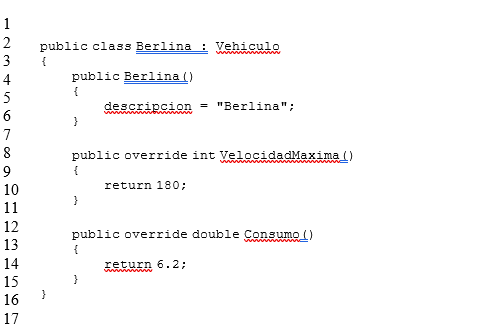
\includegraphics[width=10cm]{./Imagenes/decorator5} 
	\end{center}

Como vemos, ambas clases heredan un atributo común, “descripcion”, y la funcionalidad VelocidadMaxima y Consumo. Asumiremos que un monovolumen posee una velocidad máxima de 160km/h y un consumo de 7,5 litros/100km, mientras que una berlina podrá alcanzar los 180km/h con un consumo de 6,2 litros/100km. Esta funcionalidad será modificada por nuestras clases decoradoras, que podrán aumentar o disminuir estas características.
Con esto habríamos codificado nuestra rama “funcional”. Aún no hay rastro del patrón Decorator, ya que únicamente hemos hecho uso de la herencia de la manera habitual (de hecho, de una forma un tanto escueta).
\begin{center}
	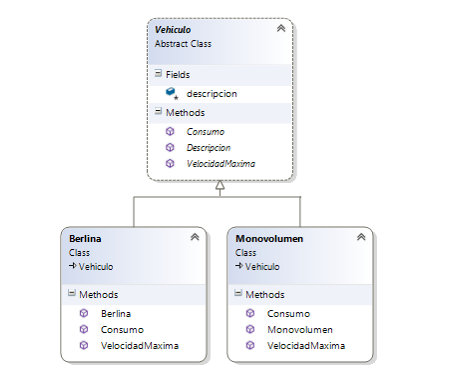
\includegraphics[width=10cm]{./Imagenes/decorator6} 
	\end{center}

\textbf{Creando las clases Decorator}

Es hora, por tanto, de añadir una nueva “rama” a nuestro árbol, añadiendo los decoradores. Comenzaremos por crear una nueva clase abstracta que herede de Vehiculo (para que pueda ocupar su lugar) y de la cual heredarán todos los decoradores.
\begin{center}
	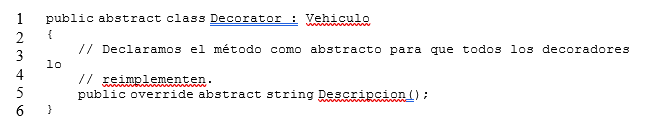
\includegraphics[width=10cm]{./Imagenes/decorator7} 
	\end{center}

A continuación añadiremos los decoradores, que incluirán una referencia a un vehículo y que se construirán mediante la inyección de éste. Por tanto, las características de estos decoradores, además de heredar de Decorator, serán las siguientes:

\begin{itemize}



  \item Contienen una referencia a un Vehiculo, que se insertará en el constructor.
  \item Modifican el funcionamiento de las clases que encapsulan, accediendo a sus atributos y métodos y adaptándolos a la nueva funcionalidad deseada.


\end{itemize} 

Comenzaremos añadiendo un decorador llamado “Gasolina”. La gasolina, al ser más explosiva, proporciona mayor velocidad punta, pero al ser menos energética que el gasoil, también conlleva tener un consumo más elevado. Esta clase tendrá, por tanto, el siguiente aspecto:

\begin{center}
	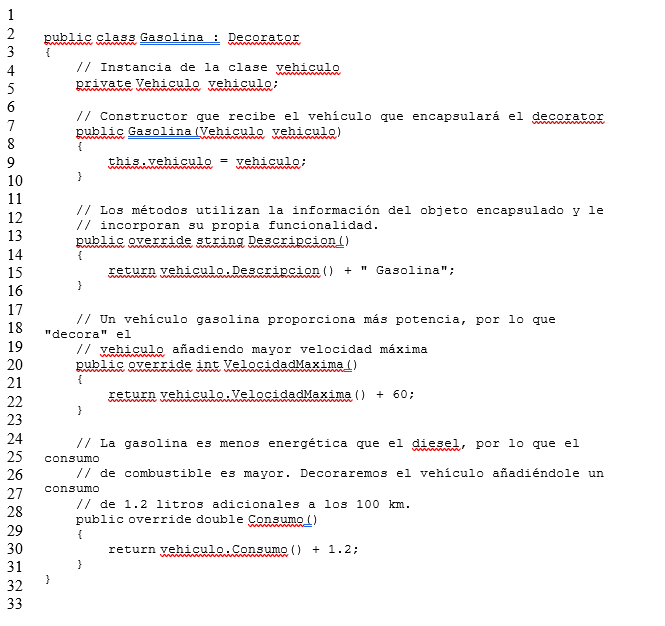
\includegraphics[width=10cm]{./Imagenes/decorator8} 
	\end{center}

Podemos utilizar un razonamiento análogo para un motor diesel, que tendrá el funcionamiento opuesto.
\begin{center}
	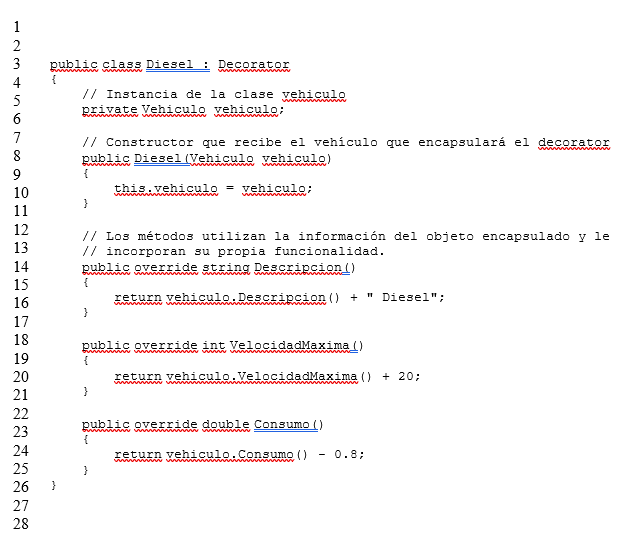
\includegraphics[width=10cm]{./Imagenes/decorator9} 
	\end{center}


¡Ojo! Según nuestro diseño, un vehículo podría ser a la vez diesel y gasolina, ya que ambos heredan de la clase Vehiculo. Las reglas de negocio no deberían permitir que esto fuera así, por lo que deberíamos utilizar reglas adicionales para evitar que ambos decoradores estuviesen presentes en un mismo objeto. No obstante, ignoraremos este hecho en este ejemplo.
A continuación añadiremos nuevos decoradores a nuestro vehículo. Por ejemplo, el turbo.

\begin{center}
	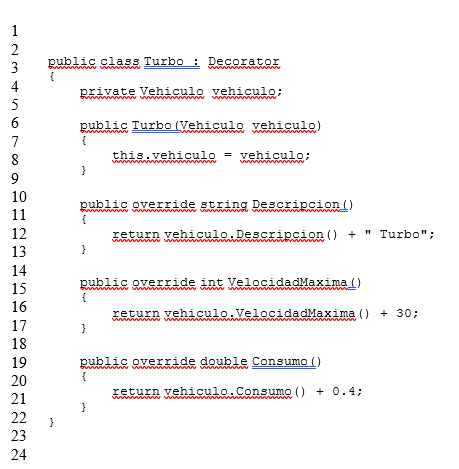
\includegraphics[width=10cm]{./Imagenes/decorator10} 
	\end{center}

Otra posible modificación al vehículo original podría ser la inyección de combustible, que no afectará a la velocidad pero mejorará notablemente el consumo de combustible:
\begin{center}
	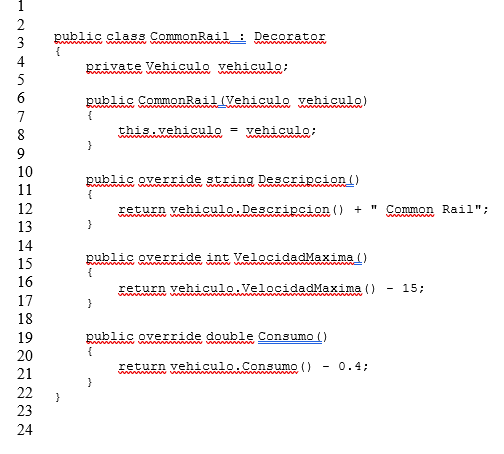
\includegraphics[width=10cm]{./Imagenes/decorator11} 
	\end{center}

Tras nuestra última adquisición, nuestra jerarquía de clases tendrá el siguiente aspecto:

\begin{center}
	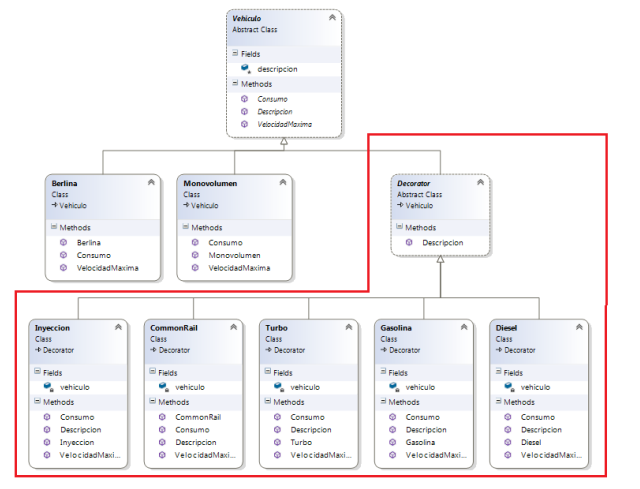
\includegraphics[width=10cm]{./Imagenes/decorator12} 
	\end{center}

Ahora es posible componer, en tiempo de ejecución, un objeto que combine algunas o todas estas características sin necesidad de codificar una clase por cada posible combinación.

\textbf{Utilizando el patrón Decorator}
Es hora de hacer uso del patrón que acabamos de explicar. Comenzaremos creando un vehículo monovolumen y otro vehículo de tipo berlina, mostrando por pantalla sus características:
\begin{center}
	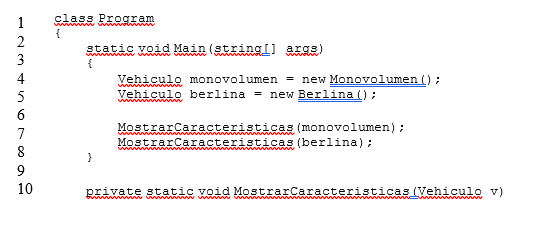
\includegraphics[width=10cm]{./Imagenes/decorator13} 
	\end{center}
\textbf{}\\ 
\begin{center}
	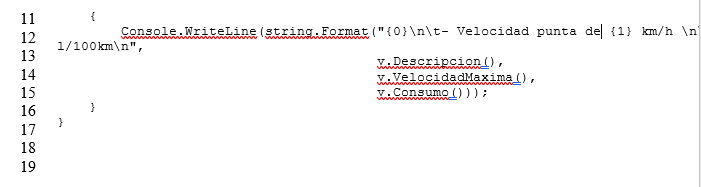
\includegraphics[width=10cm]{./Imagenes/decorator14} 
	\end{center}
\textbf{}\\ 
Nuestro programa nos mostrará el siguiente resultado:
\textbf{}\\ 
\begin{center}
	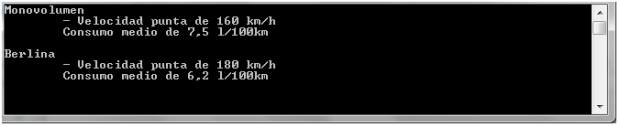
\includegraphics[width=10cm]{./Imagenes/decorator15} 
	\end{center}
\textbf{}\\ 

Como vemos, se nos ofrece una versión “básica” de nuestros objetos, que aún no han sido decorados. Probemos a decorar nuestro monovolumen añadiéndole un motor gasolina:
\textbf{}\\ 
\begin{center}
	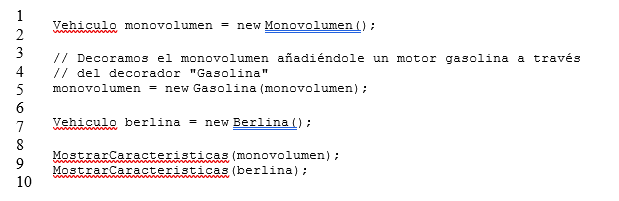
\includegraphics[width=10cm]{./Imagenes/decorator16} 
	\end{center}
\textbf{}\\ 
Esto modificará el comportamiento de nuestro monovolumen, que presentará las siguientes características:
\textbf{}\\ 
\begin{center}
	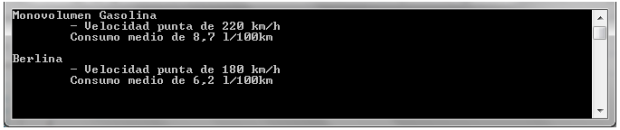
\includegraphics[width=10cm]{./Imagenes/decorator17} 
	\end{center}
\textbf{}\\ 
Se ha modificado, por tanto, su descripción, velocidad punta y consumo medio. Hagamos lo propio con el vehículo de tipo Berlina, al que convertiremos en un vehículo diesel turbo inyección common-rail:
\textbf{}\\ 
\begin{center}
	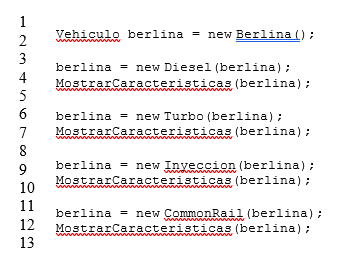
\includegraphics[width=10cm]{./Imagenes/decorator18} 
	\end{center}
\textbf{}\\ 
Como podemos observar, la propia instancia de Vehiculo es pasada como parámetro al constructor, que devuelve la misma instancia decorada con la nueva funcionalidad.
\textbf{}\\ 
\begin{center}
	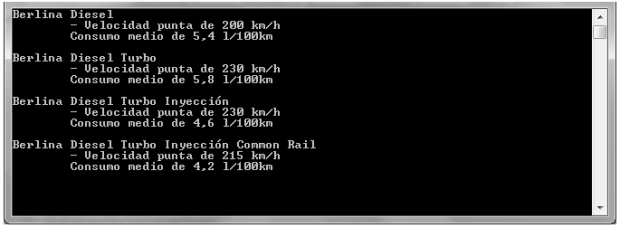
\includegraphics[width=10cm]{./Imagenes/decorator19} 
	\end{center}
\textbf{}\\ 
Así, con una única referencia, hemos conseguido modificar el comportamiento de la instancia en tiempo de ejecución sustituyendo la capacidad de especialización de la herencia por un proceso horizontal de composición.

\textbf{¿Cuándo utilizar este patrón? Ejemplos reales?}
No debemos hacer caso omiso de que la referencia “berlina” ocupará ahora en memoria el quíntuple de lo que originalmente ocupaba, ya que se trata en realidad de una referencia a CommonRail que contiene un objeto Inyeccion que contiene un objeto Turbo que contiene un objeto Diesel que a su vez contiene la instancia Berlina original. Por tanto, conviene estudiar bien el contexto en el que se utilizará este patrón, ya que el ahorro que obtendremos en diseño lo pagaremos en memoria.
\textbf{}\\ 
\begin{center}
	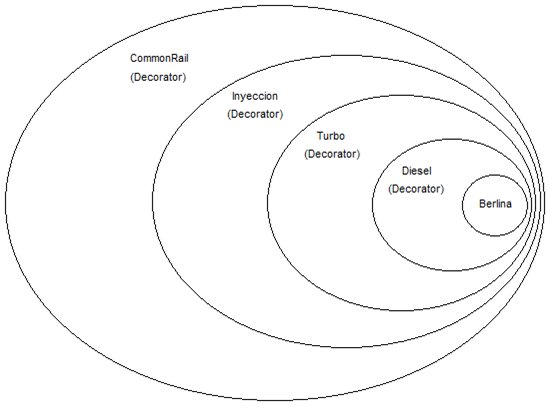
\includegraphics[width=10cm]{./Imagenes/decorator20} 
Un ejemplo claro de este patrón en la API de .NET es la familia de clases Stream. La clase Streames una clase abstracta que expone la funcionalidad básica que será implementada por las clases concretas y decoradas por las clases que componen el patrón.
	\end{center}
\textbf{}\\ 

Algunas de las clases concretas que podemos encontrar en esta familia son las siguientes:


  \item FileStream: representa un flujo (stream) que se encargará de realizar operaciones E/S sobre un fichero físico.

  \item MemoryStream: representa un flujo que realizará operaciones E/S en memoria. Se usa como una proyección temporal en memoria de otro flujo.

  \item 	BufferedStream: representa una sección de un flujo que realizará operaciones E/S en memoria. La diferencia con el anterior es que el MemoryStream representa un flujo completo (por ejemplo, una proyección en memoria de un FileStream), mientras que BufferedStream se usa en conjunción con otros Streams para realizar operaciones de E/S que posteriormente serán leídas o volcadas desde/hacia el flujo original.

Estas clases serían nuestra Berlina y Monovolumen. Pero ¿y los Decorator? Las clases que actúan como decoradores son fácilmente identificables porque reciben un Stream como parámetro a la hora de crear una nueva instancia, a la vez que extienden la funcionalidad del objeto de la clase original.
\textbf{}\\ 
Algunos de los decoradores que podemos encontrar, y que son aplicables a cualquiera de las tres clases anteriores son:

  \item 	CryptoStream: define una secuencia que vincula los flujos de datos a las transformaciones criptográficas.
  \item 	AuthenticatedStream: proporciona métodos para pasar las credenciales a través de una secuencia y solicitar o realizar la autenticación para las aplicaciones de cliente-servidor.
  \item 	GZipStream: proporciona los métodos y propiedades que permiten comprimir y descomprimir secuencias.

\textbf{}\\ 
\textbf{}\\ 
Cada uno de estos Decorator reciben en su constructor un Stream, añadiéndole nuevas funcionalidades y permitiendo que sigan actuando como Stream. Debido al polimorfismo, un CryptoStream que decore un MemoryStream seguirá pudiendo sustituir a cualquier objeto que se pase como parámetro como una referencia a Stream.
\textbf{}\\ 
\begin{center}
	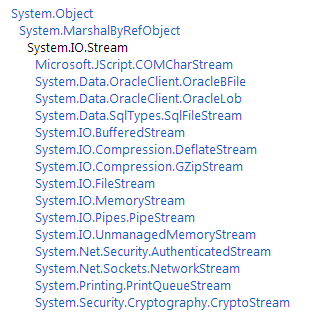
\includegraphics[width=10cm]{./Imagenes/decorator21} 

	\end{center}
\textbf{}\\ 


Podemos ver un ejemplo similar en Java, donde la clase InputStream actuaría como la clase base abstracta, clases como FileInputStream, StringBufferInputStream y ByteArrayInputStream actuarían como clases concretas, FilterInputStream actuaría como la clase abstracta de la que heredan todos los decoradores (clase que no existe en la familia Stream de .NET) y clases como BufferedInputStream, DataInputStream o LineNumberInputStream actuarían como decoradores, recibiendo un objeto de la clase InputStream como parámetro en su constructor.






\end{flushleft}
\section{Proceso de diseño de software combinado con TD} 
\textbf{}\\
\begin{flushleft}


\begin{itemize}


\item 1.El Cliente escribe su historia de usuario.

\textbf{}\\
\item 2.Se escriben junto con el cliente los criterios de aceptación de esta historia, desglosándolos mucho para simplificarlos todo lo posible.


\textbf{}\\
\item 3.Se escoge el criterio de aceptación más simple y se traduce en una prueba unitaria.

\textbf{}\\

\item 4.Se comprueba que esta prueba falla.

\textbf{}\\

\item 5.Se escribe el código que hace pasar la prueba.

\textbf{}\\

\item 6.Se ejecutan todas las pruebas automatizadas.

\textbf{}\\

\item 8.Se refactoriza y se limpia el código.

\textbf{}\\

\item 9.Se vuelven a pasar todas las pruebas automatizadas para comprobar que todo sigue funcionando.

\textbf{}\\

\item Volvemos al punto 3 con los criterios de aceptación que falten y repetimos el ciclo una y otra vez hasta completar nuestra aplicación.

	


\end{itemize} 


\end{flushleft}

\section{Patrones de Diseño Adapter} 
\textbf{}\\
\begin{flushleft}
El patrón de diseño Adapter es utilizado cuando tenemos interfaces de software incompatibles, las cuales a pesar de su incompatibilidad tiene una funcionalidad similar. Este patrón es implementado cuando se desea homogeneizar la forma de trabajar con estas interfaces incompatibles, para lo cual se crea una clase intermedia que funciona como un adaptador. Esta clase adaptador proporcionará los métodos para interactuar con la interface incompatible.


	\begin{center}
	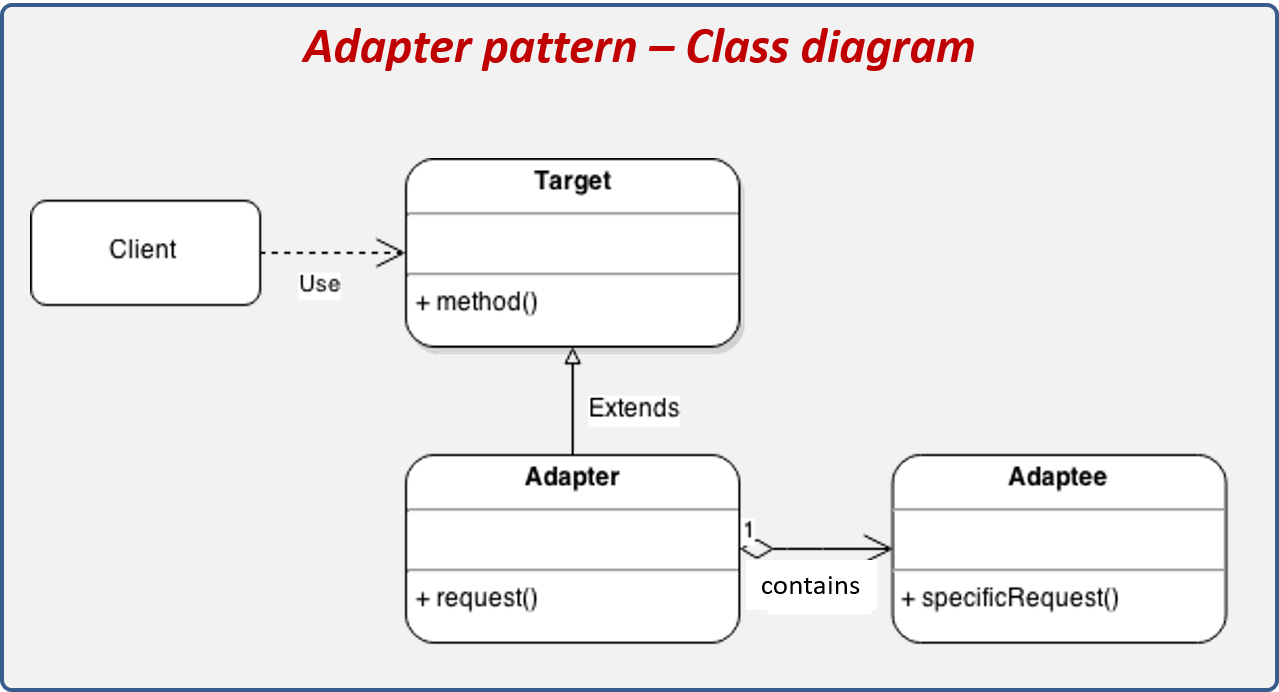
\includegraphics[width=10cm]{./Imagenes/adapter} 
	\end{center}

\textbf{  Los componentes que conforman el patrón son los siguientes:}\\
\begin{enumerate}[a)]
\item Client: Actor que interactua con el Adapter.
\item Target: Interface que nos permitirá homogenizar la forma de trabajar con las interfaces incompatibles, esta interface es utilizada para crear los Adapter.
\item Adapter: Representa la implementación del Target, el cual tiene la responsabilidad de mediar entre el Client y el Adaptee. Oculta la forma de comunicarse con el Adaptee.
\item Adaptee: Representa la clase con interface incompatible.
                                                                                                                                                                                                             
\newpage


\end{enumerate}
         \begin{center}
	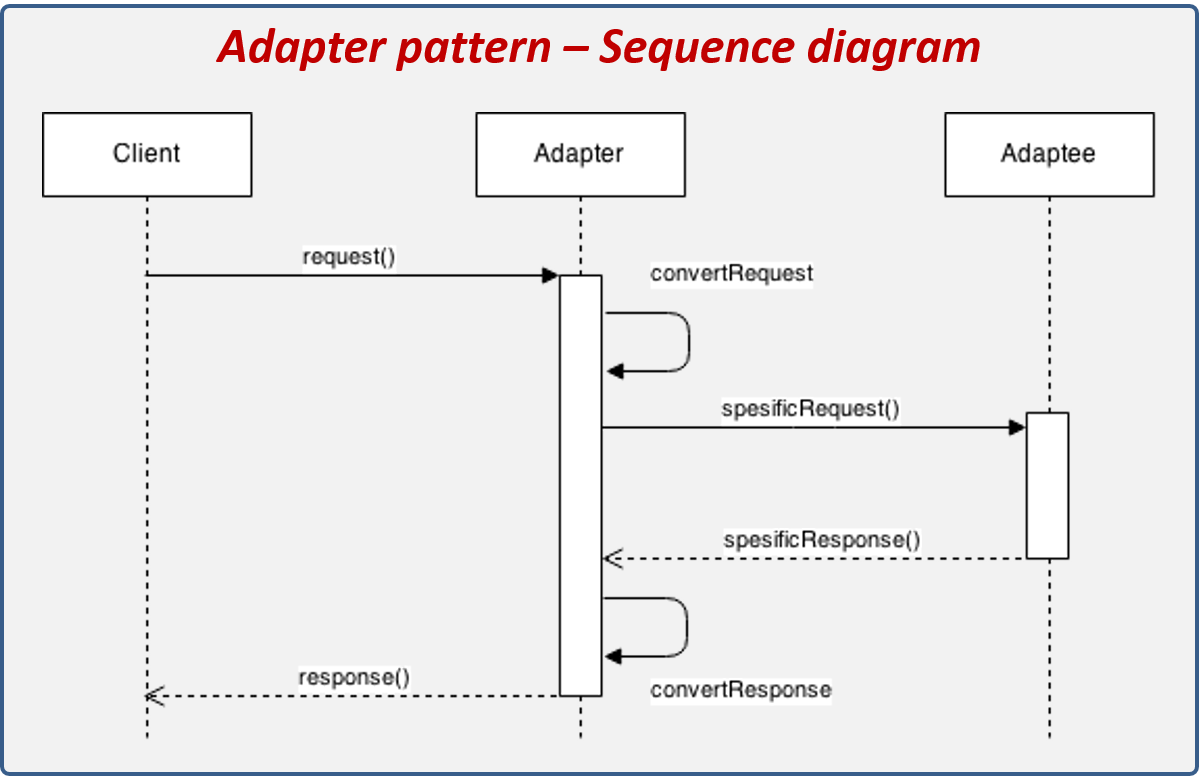
\includegraphics[width=10cm]{./Imagenes/adapter2} 
	\end{center}
\vfill

\begin{enumerate}[a)]
\item El Client invoca al Adapter con parámetros genéricos.
\item El Adapter convierte los parámetros genéricos en parámetros específicos del Adaptee.
\item El Adapter invoca al Adaptee.
\item El Adaptee responde.
\item El Adapter convierte la respuesta del Adaptee a una respuesta genérica para el Client.
\item El Adapter responde al Client con una respuesta genérica.
\end{enumerate}
\vfill
\textbf{         EJEMPLO DEL MUNDO REAL}
\\ Mediante la implementación del patrón de diseño Adapter crearemos un adaptador que nos permite interactuar de forma homogénea entre dos API bancarías, las cuales nos permite aprobar créditos personales, sin embargo, las dos API proporcionadas por los bancos cuenta con interfaces diferentes y aunque su funcionamiento es prácticamente igual, las interfaces expuestas son diferentes, lo que implica tener dos implementaciones diferentes para procesar los préstamos con cada banco. Mediante este patrón crearemos un adaptador que permitirá ocultar la complejidad de cada implementación del API, exponiendo una única interface compatible con las dos API proporcionadas, además que dejáramos el camino preparado por si el día de mañana llegara una nueva API bancaría.
          \begin{center}
	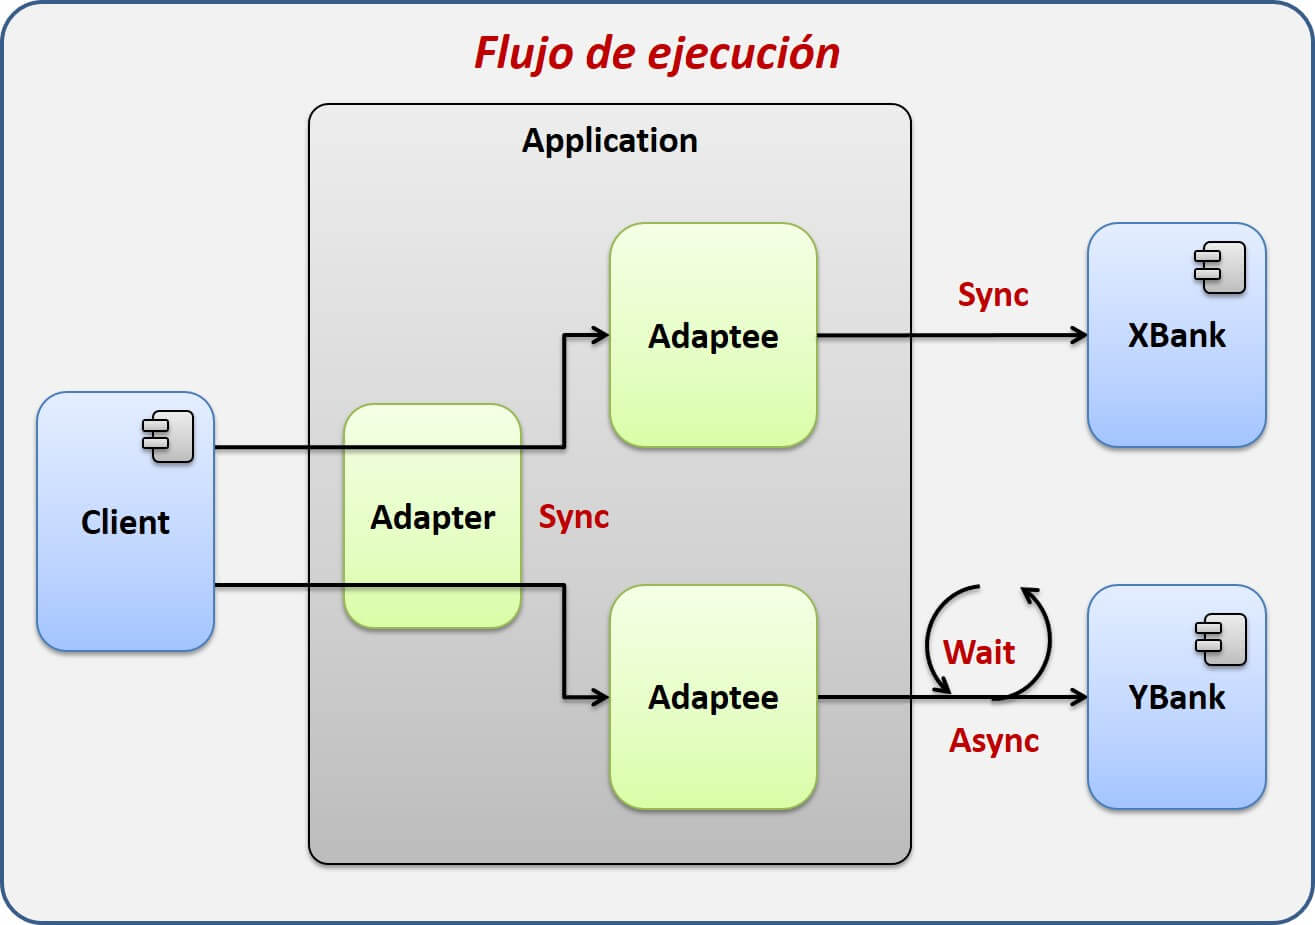
\includegraphics[width=10cm]{./Imagenes/adapter3} 
	\end{center}
	




\end{flushleft}

\section{Ventajas del TDD, Posibles problemas del TDD y Sus Soluciones} 
\textbf{}\\

\begin{flushleft}
\begin{itemize}
\textbf{1.   Ventajas del TDD}
\textbf{}\\
\textbf{- Mayor calidad }

Garantiza que las pruebas se ejecutan (no sean omitidas), evitando que las aplicaciones tengan fallas la primera vez que el usuario las ejecuta o que el usuario encuentre los errores, en lugar de ser encontrados por el equipo de desarrollo. \textbf{}\\
Asimismo, el hacer pruebas en etapas tempranas del desarrollo es una forma de incorporar la calidad al proceso, resultando en menos errores (bugs) en las etapas finales del proyecto. 

\textbf{}\\
\textbf{- Diseño enfocado en las necesidades }

El escribir las pruebas primero que el código, obliga a que las necesidades reales del cliente sean consideradas primero, obligando a analizar primero qué es lo que realmente se necesita que el código haga y no al contrario. Como resultado, habrá menos retrabajo después. 
\textbf{}\\
\textbf{- Mayor simplicidad en el diseño  }

El escribir las pruebas primero que el código, obliga a que las necesidades reales del cliente sean consideradas primero, obligando a analizar primero qué es lo que realmente se necesita que el código haga y no al contrario. Como resultado, habrá menos retrabajo después. 

\textbf{}\\
\textbf{- Mayor simplicidad en el diseño  }

Bajo TDD, en lugar de enfocarse en realizar diseños extensos y complejos, el equipo se enfocará en la necesidad o requerimiento del cliente, agregando solamente la funcionalidad que el cliente necesita. Esto es muy importante, pues es la complejidad la que produce los errores. \textbf{}\\

Esto obliga a escribir código enfocado en las necesidades del usuario, evitando antipatrones como los objetos multipropósito (clase gorda) o el acoplamiento del código, dado que desarrollarán códigos específicos a los requerimientos que se estén atendiendo en esa iteración. 
\textbf{}\\
\textbf{- El diseño se va adaptando al entendimiento del problema }

A medida que se realizan iteraciones de probar y programar, el entendimiento del problema se incrementa, de esta forma, sucesivas iteraciones cuentan con un mayor entendimiento, lo que reduce los malos entendidos de la funcionalidad al final del desarrollo, resultando en menos retrabajo. 

\textbf{}\\
\textbf{- Mayor productividad  }
En un proyecto tradicional, generalmente lo que sucede es que al principio se es muy productivo, sin embargo, esa productividad cae hacia el final del proyecto, cuando empiezan a encontrarse errores en todas partes, se encuentran malentendidos en lo que el cliente quería, o cuando el cliente hace un par de cambios desestabilizadores. \textbf{}\\

En contraposición a este esquema, una de las principales ventajas de TDD es que se obtiene retroalimentación (feedback) inmediato sobre el software desarrollado. \textbf{}\\

Trabajando bajo TDD, al principio se algo improductivo, pues se necesita escribir una serie de casos de prueba que fallaran al primer intento, sin embargo, los beneficios se hacen evidentes cuando se ha probado constantemente la aplicación, se han corregido los errores de forma temprana y de han aclarado de forma temprana las dudas en la funcionalidad.

\textbf{}\\
\textbf{- Menos tiempo invertido en debugging de errores }

El código se va desarrollando por piezas pequeñas, por ende, cuando surge un error, los esfuerzos se enfocan en la pequeña pieza de código que fue modificada, por lo que se le pueden llegar a los problemas de forma más directa. 

\textbf{2.   Posibles problemas del TDD y sus soluciones }
\textbf{}\\

\textbf{- Interfaz de usuario}
\textbf{}\\
TDD es difícil de implementar en la capa de interfaz de usuario (presentación), debido a que está actividad contiene elementos que contienen a alargar el ciclo de prueba y desarrollo. En su lugar, TDD encaja más fácilmente en los desarrollos en las capas de lógica de negocios (objetos y dominio) y acceso a datos. Por ende, pueden existir reservas respecto a aplicar TDD en una aplicación con alto grado de interacción con el usuario. 

Sin embargo, esto no es necesariamente algo malo, dado que la metodología obliga a separar las capas y a no implementar lógica de negocio en la capa de presentación, lo cual sería un anti patrón. 

\textbf{- La Base de datos }
\textbf{}\\
Uno de los principales problemas de usar TDD en aplicaciones con bases de datos, es que una vez que se ha ejecutado una prueba, la base de datos puede quedar en un estado distinto al que se necesita para hacer la siguiente prueba (por ejemplo, si la aplicación necesita cambiar el valor de un campo de A a B, cuando la prueba termina el valor queda en B, por lo que no se puede ejecutar una siguiente prueba). \textbf{}\\

Una forma de abordar este problema es escribir código para inicializar la base de datos en el estado previo, sin embargo esto añade carga de trabajo adicional. \textbf{}\\

Otra solución es utilizar objetos para representar la base de datos, por medio de objetos cascaron, respuestas predefinidas o dummies que emulen las respuestas de la base de datos. 

\textbf{- Errores no identificados }
\textbf{}\\

Sólo por el hecho de pasar todas las pruebas en la herramienta que se utilize (JUNIT por ejemplo), no significa que no se tengan errores, sólo significa que las pruebas que se han ejecutado no han encontrado errores. El utilizar TDD podría llevar a un falso sentimiento de seguridad, por ende, se necesita enfocarse en que las pruebas sean detalladas y cubran todos los escenarios posibles. 

\textbf{-  Perder la visión general (Ver el árbol en lugar del bosque)  }
\textbf{}\\
TDD es un enfoque de abajo hacia arriba (Bottom-Up), y se debe estar al tanto que podría perderse visibilidad general del proyecto y del aplicativo. Es una buena idea mantener un modelo general (bajo un enfoque tradicional como UML) y revisarlo de vez en cuanto, quizás se encuentren oportunidades para refactorizar y hacer que la aplicación se le pueda dar mantenimiento en el tiempo. 
\textbf{-  Pronunciada curva de aprendizaje }
Como se ha dicho en otras entregas, TDD es difícil de adoptar, por lo que puede esperarse un descenso en la productividad durante los primeros dos meses de implementación. Lo recomendable para enfrentar esto es buscar ayuda, por medio de formación (cursos) y consultorías que apoyen en la adopción de la nueva forma de trabajo. 

\end{itemize} 



\end{flushleft}
\section{Webgrafía} 
\textbf{}\\
\begin{flushleft}

\begin{itemize}

	\item https://uniwebsidad.com/libros/tdd/capitulo-2
           \item https://docs.microsoft.com/es-es/previous-versions/bb932285(v=msdn.10)
           \item http://www.conaiisi.unsl.edu.ar/portugues/2013/158-524-1-DR.pdf
           \item https://openwebinars.net/blog/que-es-tdd-test-driven-development/
           \item https://altenwald.org/2009/01/08/desarrollo-orientado-a-pruebas-tdd/
           \item https://uniwebsidad.com/libros/tdd/capitulo-2


\end{itemize} 


\end{flushleft}


\end{document}